\documentclass[14pt]{beamer}

% Presento style file
\usepackage{config/presento}
% custom command and packages
% custom packages
\usepackage{textpos}
\setlength{\TPHorizModule}{1cm}
\setlength{\TPVertModule}{1cm}

\newcommand\crule[1][black]{\textcolor{#1}{\rule{2cm}{2cm}}}



% Custom colors
\usepackage{color}
\definecolor{ao}{rgb}{0.0, 0.5, 0.0}


% Information
\title{LOST IN HYPERSPACE}
\subtitle{\emph{The Curse of Dimensionality}}
\author{Zachary del Rosario}
\institute{zdr@stanford.edu}
\date{September 6th}
%% \date{\today}

% --------------------------------------------------
\begin{document}
% --------------------------------------------------

% --------------------------------------------------
\framecard[colorgreen]{{\color{white}\hugetext{%
      \centering%
      Please print your\\
      name on a card!
}}}

% -------------------------
\begin{frame}[plain]
\maketitle
\end{frame}

% -------------------------
\framepicv[1.0]{images/olin_compressed}{} % Olin

% -------------------------
\framepicv[1.0]{images/seq}{} % Stanford Engineering Quad

% -------------------------
\framepicv[1.0]{images/lax_shuttle-25p}{
 \begin{textblock}{7}(0.0,5.7)
    {\tiny By Aaron Barnaby aaronbarnaby}
 \end{textblock}
}

% -------------------------
\framepicv[0.8]{images/gipsy_moth-25p}{
 \begin{textblock}{7}(0.0,5.7)
    {\tiny By Peripitus - Own work, CC BY-SA 3.0}
 \end{textblock}%
 \textblockcolor{white}
 \textblockrulecolor{black}
 \only<2>{
   \begin{textblock}{4.5}(0.0,3.5)
     {
       \begin{tabular}{l|l}
       \hline
       Strength & Spar1\\
       \hline
       Stress? & Size?\\
       \hline
       \end{tabular}
     }
   \end{textblock}
 }%
 \only<3>{
   \begin{textblock}{6.2}(0.0,3.5)
     {
       \begin{tabular}{l|l|l}
       \hline
       Strength & Spar1 & Spar2\\
       \hline
       Stress? & Size? & Size?\\
       \hline
       \end{tabular}
     }
   \end{textblock}
 }%
 \only<4>{
   \begin{textblock}{11.0}(0.0,3.5)
     {
       \begin{tabular}{l|l|l|l|l|l}
       \hline
       Strength & Spar1 & Spar2 & Rib1 & Rib2 & Rib3\\
       \hline
       Stress? & Size? & Size? & Size? & Size? & Size?\\
       \hline
       \end{tabular}
     }
   \end{textblock}
 }%
 \textblockcolor{}
 \textblockrulecolor{}
}

% -------------------------
\begin{frame}[plain]
 \textblockcolor{}
 \textblockrulecolor{}
  \only<1>{%
    \begin{textblock}{11}(-0.5,-1.5)
      {\textblockcolour{}
        \small
        \begin{tabular}{l|r}
        \hline
        Str & Spar1\\
        \hline
        ? & 1\\
        \hline
        ? & 2\\
        \hline
        ? & 3\\
        \hline
        \end{tabular}
      }
    \end{textblock}
    \begin{tikzpicture}[remember picture,overlay]
      \node[xshift=+3cm,yshift=+1.5cm] at (current page.center){%
        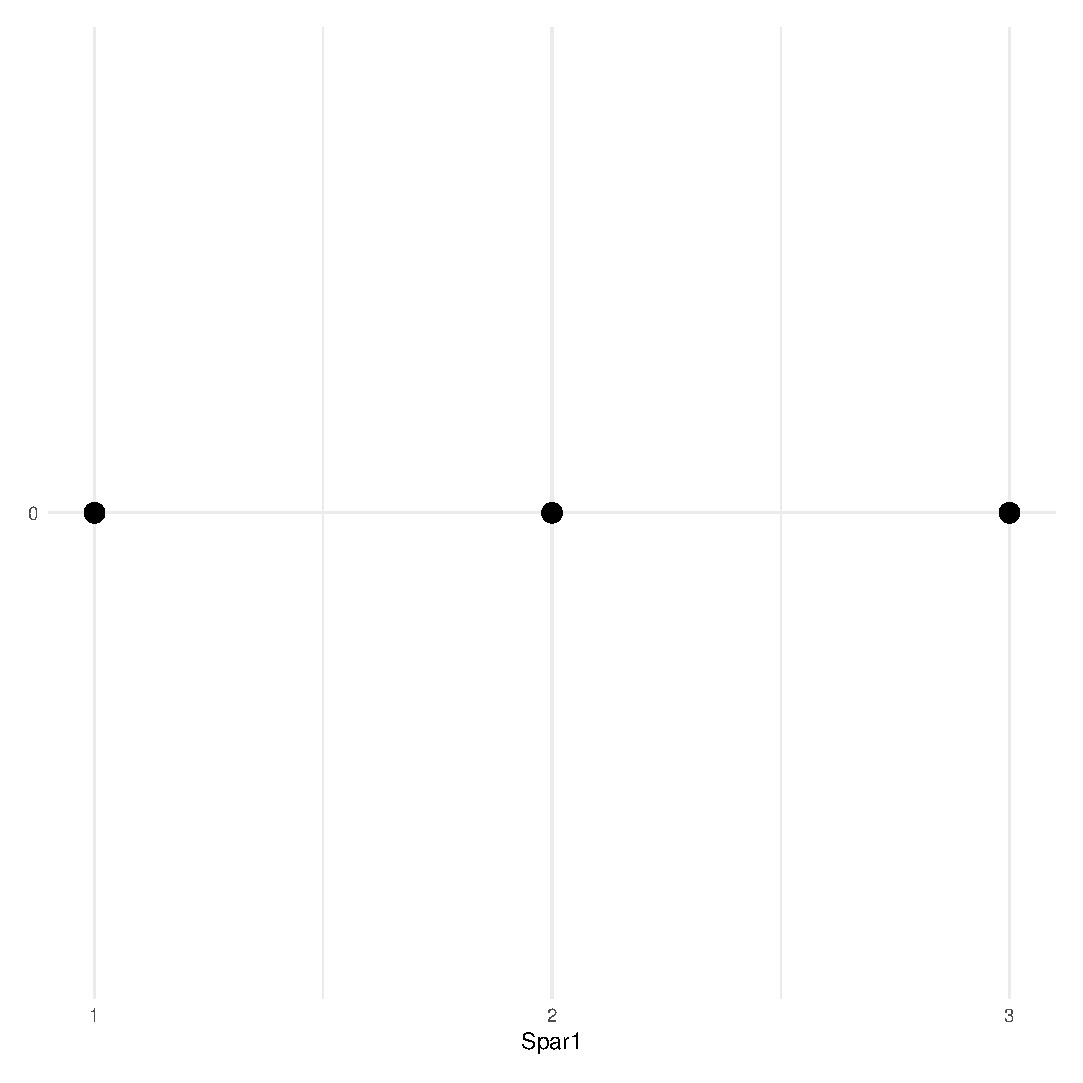
\includegraphics[width=6cm]{./images/points1}};
    \end{tikzpicture}
  }
  \only<2>{%
    \begin{textblock}{11}(-0.5,-1.5)
      {\textblockcolour{}
        \small
        \begin{tabular}{l|r|r}
        \hline
        Str & Spar1 & Spar2\\
        \hline
        ? & 1 & 1\\
        \hline
        ? & 2 & 1\\
        \hline
        ? & 3 & 1\\
        \hline
        ? & 1 & 2\\
        \hline
        ? & 2 & 2\\
        \hline
        ? & 3 & 2\\
        \hline
        ? & 1 & 3\\
        \hline
        ? & 2 & 3\\
        \hline
        ? & 3 & 3\\
        \hline
        \end{tabular}
      }
    \end{textblock}
    \begin{tikzpicture}[remember picture,overlay]
      \node[xshift=+3cm,yshift=+1.5cm] at (current page.center){%
        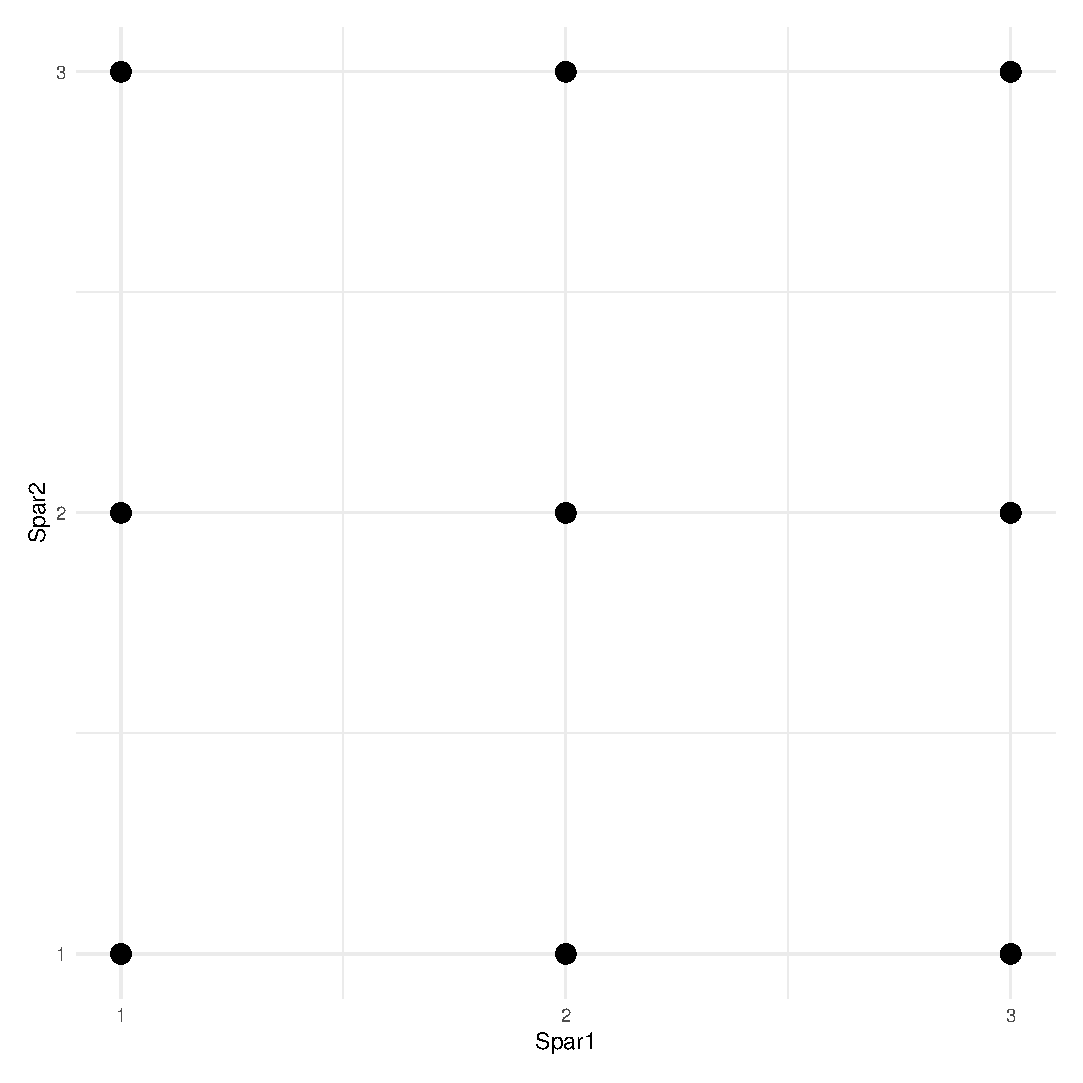
\includegraphics[width=6cm]{./images/points2}};
    \end{tikzpicture}
  }
  \only<3->{%
    \begin{textblock}{11}(-0.5,-1.5)
      {\textblockcolour{}
        \small
        \begin{tabular}{l|r|r|r}
        \hline
        Str & Spar1 & Spar2 & Rib1\\
        \hline
        ? & 1 & 1 & 1\\
        \hline
        ? & 2 & 1 & 1\\
        \hline
        ? & 3 & 1 & 1\\
        \hline
        ? & 1 & 2 & 1\\
        \hline
        ? & 2 & 2 & 1\\
        \hline
        ? & 3 & 2 & 1\\
        \hline
        ? & 1 & 3 & 1\\
        \hline
        ? & 2 & 3 & 1\\
        \hline
        ? & 3 & 3 & 1\\
        \hline
        \vdots & \vdots & \vdots & \vdots
        \end{tabular}
      }
    \end{textblock}
    \begin{tikzpicture}[remember picture,overlay]
      \node[xshift=+3cm,yshift=+1.5cm] at (current page.center){%
        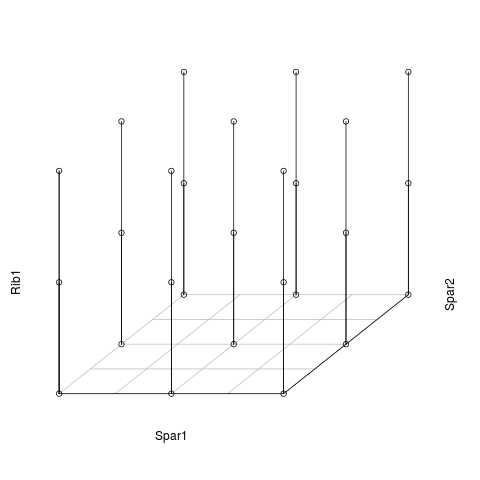
\includegraphics[width=6cm]{./images/points3}};
    \end{tikzpicture}
  }
  % Annotation
  \only<4->{
    \begin{textblock}{5}(5.5,2.5)
      {\textblockcolor{}
        That's a lot of planes! \\
        \only<5>{%
          \alert{Make a prediction:} How many planes for $d$ variables?\\
          Maybe $\approx d$? $\approx d^2$?
        }
      }
    \end{textblock}
  }
\end{frame}

% -------------------------
\framepich[0.8]{images/full_747}{
 \begin{textblock}{7}(0.0,5.7)
    {\tiny Jameson et al. (1986)}
 \end{textblock}
}

% -------------------------
\framepich[0.7]{images/titan_render}{
  \only<2>{
    \begin{textblock}{7}(0.0,4.5)
      {Simulations run\\ hours to \emph{months}}
    \end{textblock}
  }
}

% -------------------------
\begin{frame}[t]{Thought Experiment}
  Suppose our simulation ran in \emph{one second}, \\
  and we use $10$ points per dimension....

  \bigskip
  \only<2->{How long would this take to execute?\\}
  \only<3>{%
    Scaling is \emph{exponential}, i.e.
    \begin{equation*}
      \text{Time} = C^d
    \end{equation*}
  }
\end{frame}

% -------------------------
\framepicv[0.8]{images/dimensionality}{
  \only<2>{%
    \begin{textblock}{7}(3.8,3.0)
        {\textblockcolor{}
          \alert{The Curse of Dimensionality}
        }
    \end{textblock}
  }
}

% -------------------------
\begin{frame}{Outline}
  \begin{itemize}
  \item 1. \emph{Accursed} Data
  \item 2. \emph{Accursed} Geometry
  \item 3. Lifting the Curse...
  \item 4. An Activity
  \end{itemize}
\end{frame}

% --------------------------------------------------
\framecard[colorgreen]{{\color{white}\hugetext{%
      \centering%
      Big Data\\
      and\\
      Dimensionality
}}}

% -------------------------
\begin{frame}{The Data Matrix}
  We've already seen one of these!

  \begin{table}
    \begin{tabular}{l|r|r|r}
      \hline
      Str & Spar1 & Spar2 & Rib1\\
      \hline
      ? & 1 & 1 & 1\\
      \hline
      ? & 2 & 1 & 1\\
      \hline
      ? & 3 & 1 & 1\\
      \hline
      ? & 1 & 2 & 1\\
      \hline
      ? & 2 & 2 & 1\\
      \hline
      ? & 3 & 2 & 1\\
      \hline
      ? & 1 & 3 & 1\\
      \hline
      ? & 2 & 3 & 1\\
      \hline
      ? & 3 & 3 & 1\\
      \hline
      \vdots & \vdots & \vdots & \vdots
    \end{tabular}
  \end{table}
\end{frame}

% -------------------------
\begin{frame}{The Data Matrix}

  \begin{table}
    \begin{tabular}{@{}l|l|l|l@{}}
                      & Variable $1$ & $\cdots$ & Variable $d$ \\
      \hline
      Observation $1$ & $\vdots$     & $\vdots$ & $\vdots$ \\
      $\vdots$        & $\vdots$     & $\vdots$ & $\vdots$
    \end{tabular}
  \end{table}
\end{frame}

% -------------------------
\begin{frame}{A Wider Shade of Big}
  (Big data -- Dimensionality is one direction)
\end{frame}

% --------------------------------------------------
\framecard[colorgreen]{{\color{white}\hugetext{%
      \centering%
      Weird Facts\\
      about\\
      High-\\
      Dimensional\\
      Geometry
}}}

% -------------------------
\begin{frame}{Fact 1}
  Basic solids defy intuition
\end{frame}

% -------------------------
\begin{frame}{Hypercube}
  All points between intervals
\end{frame}

% -------------------------
\begin{frame}{Hypercube}
  Distance from origin to boundary

  \begin{tabular}{@{}ll@{}}
    Min & $1/2$ \\
    Max & $\sqrt{d/2}$
  \end{tabular}
\end{frame}

% -------------------------
\begin{frame}{Hypersphere}
  All points within a fixed distance
\end{frame}

% -------------------------
\begin{frame}{Hypersphere}
  Distance from origin to boundary

  \begin{tabular}{@{}ll@{}}
    Min & $1$ \\
    Max & $1$
  \end{tabular}
\end{frame}

% -------------------------
\framepich[1.0]{images/box_in_sphere1}{
 \begin{textblock}{7}(0.0,5.7)
    {\tiny By Venkatesan Guruswami}
 \end{textblock}
}
\framepich[1.0]{images/box_in_sphere2}{
 \begin{textblock}{7}(0.0,5.7)
    {\tiny By Venkatesan Guruswami}
 \end{textblock}
}
\framepich[1.0]{images/box_in_sphere3}{
 \begin{textblock}{7}(0.0,5.7)
    {\tiny By Venkatesan Guruswami}
 \end{textblock}
}

% -------------------------
\begin{frame}{Fact 2}
  The hypersphere has vanishing interior
\end{frame}

% -------------------------
\begin{frame}{Unit Hypersphere Volume}
  \begin{equation*} \begin{aligned}
      HV &= \frac{\pi ^ {d / 2}}{\Gamma(d / 2 + 1)}\\
      \visible<2>{%
        &= \int\cdots\int \alert{r^{d-1}}\,
           T(\varphi_{1},\dots,\varphi_{d-1})\,
           dr d\varphi_{1}\cdots d\varphi_{d-1}
      }
  \end{aligned} \end{equation*}
\end{frame}

% -------------------------
\framepicv[0.8]{images/surface_density}{}

% -------------------------
\begin{frame}{Fact 3}
  Johnson-Lindenstrauss....
\end{frame}

% --------------------------------------------------
\framecard[colorgreen]{{\color{white}\hugetext{%
      \centering%
      Lifting\\
      the\\
      Curse
}}}

% --------------------------------------------------
\framecard[colorgreen]{{\color{white}\hugetext{%
      \centering%
      Activity!
}}}

\end{document}
